\chapter [Sprawozdanie 2]{Opis elementów projektu} 
\fancyhead[L]{}
\fancyhead[C]{OPIS  ELEMENTÓW PROJEKTU}
\fancyhead[R]{}
\textbf{Problem (zdefiniowany na podstawie \cite{prim2}):}\\
Znalezienie takiego podzbioru krawędzi spójnego grafu nieskierowanego ważonego, który zapewnia połączenie każdego wierzchołka grafu z dowolnym innym i ponadto posiada najmniejszą możliwą sumę wag krawędzi. \\Taki podzbiór nie może zawierać żadnego cyklu, a zatem jest drzewem i musi zawierać dokładnie \emph{n-1} krawędzi dla grafu o \emph{n} wierzchołkach. Drzewo takie ze względu na minimalną sumę wag nazywane jest minimalnym drzewem rozpinającym.

\section{Algorytm Prima}
\textbf{Dane wejściowe:} \\ 
Spójny ważony graf nieskierowany, zawierający n wierzchołków, gdzie $n \geqslant 2$.\\
prim2
\subsection{Pseudokod zaimplementowanego algorytmu}
Pseudokod oraz implementację opracowano na podstawie \cite{prim2} oraz \cite{prim}.
\begin{enumerate}
	\item Inicjalizacja
	\begin{itemize}
		\item Utwórz pusty stos krawędzi MST: \emph{minSpanningTree}.
		\item Zainicjalizuj pustą kolejkę priorytetową krawędzi osiągalnych przez MST:\\ \emph{adjacencyEdges}
		\item Utwórz tablicę odwiedzonych wierzchołków grafu i ustaw wartości jej pól na \emph{false}
	\end{itemize}
	
	\item Losuj wierzchołek początkowy: \emph{startVertex}.
	\item Oznacz wierzchołek \emph{startVertex} jako odwiedzony poprzez zmianę pola tablicy o indeksie \emph{startVertex} na \emph{true}
	\item Dodaj do kolejki priorytetowej \emph{adjacencyEdges} krawędzie incydentne do odwiedzonego wierzchołka początkowego
	
	\item Powtarzaj dopóki kolejka priorytetowa \emph{adjacencyEdges} nie będzie pusta:
	\begin{itemize}
		\item[a.] Pobierz z kolejki \emph{adjacencyEdges} krawędź o najniższym koszcie
		\item[b.] Jeśli wierzchołki początkowy \emph{startVertex} i końcowy \emph{endVertex} pobranej krawędzi zostały już odwiedzone, to pomiń tę iterację i przejdź do podpunktu \textbf{a.} W przeciwnym wypadku przejdź do \textbf{c.}
		\item[c.]  Dodaj pobraną krawędź do drzewa \emph{minSpanningTree}
		\item [d.] Jeśli wierzchołek początkowy pobranej krawędzi nie został odwiedzony, to oznacz go jako odwiedzony i dodaj do kolejki \emph{adjacencyEdges} krawędzie incydentne do tego wierzchołka
		\item [e.] Jeśli wierzchołek końcowy pobranej krawędzi nie został odwiedzony, to oznacz go jako odwiedzony  i dodaj do kolejki \emph{adjacencyEdges} krawędzie incydentne do tego wierzchołka
	\end{itemize}

\item Jeśli kolejka priorytetowa już nie zawiera krawędzi, to otrzymany stos  \emph{minSpanningTree} reprezentuje otrzymane minimalne drzewo rozpinające MST
\end{enumerate} 


%%%%%%%%%%%%%%%%%%%%%%%%%%%%%%%%%
\newpage
\subsection{Zasada działania zaimplementowanego algorytmu na przykładzie}
Poniżej znajduje się legenda oznaczeń wykorzystanych w opisie działania algorytmu na przykładzie.

\begin{figure}[htb!]
	\centering
	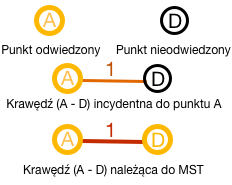
\includegraphics[width=0.4\textwidth]{tex/fig/legenda}
	\caption{Oznaczenia wykorzystane w opisie}
	\label{fig: legenda}
\end{figure}

Dany jest graf widoczny na rys.\ref{fig: g1}.  Wierzchołki oznaczono wielkimi literami alfabetu,\\ natomiast krawędziom nadano wagi $w\subseteq \{1,5\}$.\\

\begin{figure}[htb!]
	\centering
	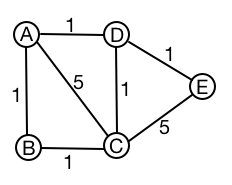
\includegraphics[width=0.4\textwidth]{tex/fig/graf1}
	\caption{Graf wejściowy.}
	\label{fig: g1}
\end{figure}

\newpage
\textbf{Inicjalizacja}\\
Stos: \emph{minSpanningTree} =\{ \};\\
Tablica wierzchołków odwiedzonych: \emph{visitedVertices} = [ false, false, false, false, false ];\\
Kolejka priorytetowa krawędzi incydentnych: \emph{adjacencyEdges} = [ ];

\textbf{Krok 1.}\\
Losowanie wierzchołka początkowego. W tym przypadku niech będzie to wierzchołek \textbf{A}.
\begin{center}
	\emph{startVertex} = A
\end{center}

\textbf{Krok 2.}\\
Oznaczenie wierzchołka \emph{startVertex} jako odwiedzony oraz dodanie jego krawędzi incydentnych do kolejki priorytetowej. 
\begin{figure}[htb!]
	\centering
	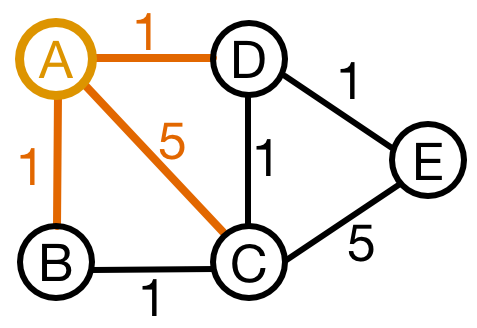
\includegraphics[width=0.4\textwidth]{tex/fig/graf2}
	\caption{Prim -- Krok 2.}
	\label{fig: g2}
\end{figure}\\
Stos: \emph{minSpanningTree} =\{ \};\\
Tablica wierzchołków odwiedzonych: \emph{visitedVertices} = [ true, false, false, false, false ];\\
Kolejka priorytetowa krawędzi incydentnych: \emph{adjacencyEdges} = [ (A - D), (A - B), (A - C)];\\

\textbf{Krok 3.}\\
Pobranie z kolejki krawędzi (A - D). Jej wierzchołek końcowy nie jest jeszcze odwiedzony, więc krawędź ta zostaje dodana do \emph{minSpanningTree}. Wierzchołek końcowy tej krawędzi - D - zostaje oznaczony jako odwiedzony, a jego krawędzie incydentne zostają dodane do kolejki \emph{adjacencyEdges} .
\begin{figure}[htb!]
	\centering
	
\includegraphics[width=0.4\textwidth]{tex/fig/graf3}
	\caption{Prim -- Krok 3.}
	\label{fig: g3}
\end{figure}\\
Stos: \emph{minSpanningTree} =\{ (A - D)\};\\
Tablica wierzchołków odwiedzonych: \emph{visitedVertices} = [ true, false, false, true, false ];\\
Kolejka priorytetowa krawędzi incydentnych:\\ \emph{adjacencyEdges} = [ (A - B), (D - E), (D - C), (A - C) ];\\

\textbf{Krok 4.}\\
Pobranie z kolejki krawędzi (A - B). Jej wierzchołek końcowy nie jest jeszcze odwiedzony, więc krawędź ta zostaje dodana do \emph{minSpanningTree}. Wierzchołek końcowy tej krawędzi - B - zostaje oznaczony jako odwiedzony, a jego krawędzie incydentne zostają dodane do kolejki \emph{adjacencyEdges} .
\begin{figure}[htb!]
	\centering
	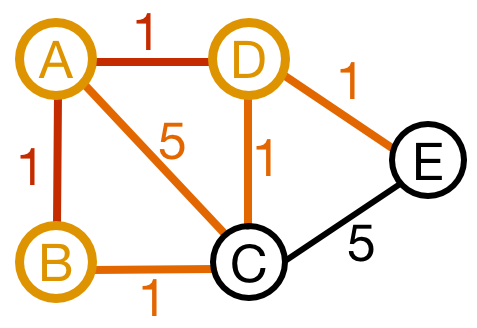
\includegraphics[width=0.4\textwidth]{tex/fig/graf4}
	\caption{Prim -- Krok 4.}
	\label{fig: g4}
\end{figure}\\
Stos: \emph{minSpanningTree} =\{ (A - B), (A - D) \};\\
Tablica wierzchołków odwiedzonych: \emph{visitedVertices} = [ true , true, false, true, false];\\
Kolejka priorytetowa krawędzi incydentnych: \\ \emph{adjacencyEdges} = [ (D - E), (D - C), (B - C), (A - C) ];\\

\textbf{Krok 5.}\\
Pobranie z kolejki krawędzi (D - E). Jej wierzchołek końcowy nie jest jeszcze odwiedzony, więc krawędź ta zostaje dodana do \emph{minSpanningTree}. Wierzchołek końcowy tej krawędzi - E - zostaje oznaczony jako odwiedzony, a jego krawędzie incydentne zostają dodane do kolejki \emph{adjacencyEdges} .
\begin{figure}[htb!]
	\centering
	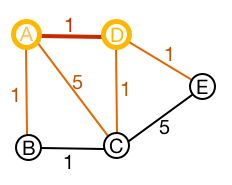
\includegraphics[width=0.4\textwidth]{tex/fig/graf5}
	\caption{Prim -- Krok 5.}
	\label{fig: g5}
\end{figure}\\
Stos: \emph{minSpanningTree} =\{ (D - E), (A - B), (A - D) \};\\
Tablica wierzchołków odwiedzonych: \emph{visitedVertices} = [ true , true, false, true, true];\\
Kolejka priorytetowa krawędzi incydentnych: \\ \emph{adjacencyEdges} = [ (D - C), (B - C), (A -- C), (E - C) ];\\

\textbf{Krok 6.}\\
Pobranie z kolejki krawędzi (D - C). Jej wierzchołek końcowy nie jest jeszcze odwiedzony, więc krawędź ta zostaje dodana do \emph{minSpanningTree}. Wierzchołek końcowy tej krawędzi - C - zostaje oznaczony jako odwiedzony. Jego krawędzie incydentne nie zostają jednak dodane do kolejki \emph{adjacencyEdges}, ponieważ ich wierzchołki końcowe zostały już odwiedzone.
\begin{figure}[htb!]
	\centering
	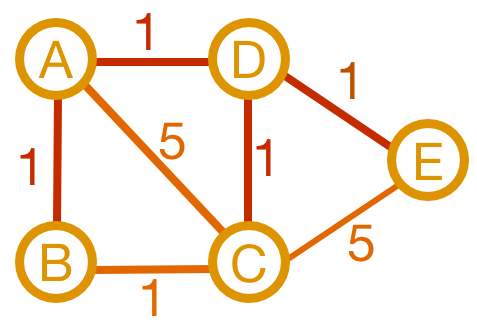
\includegraphics[width=0.4\textwidth]{tex/fig/graf6}
	\caption{Prim -- Krok 6.}
	\label{fig: g6}
\end{figure}\\
Stos: \emph{minSpanningTree} =\{ (D - C), (D - E), (A - B), (A - D) \};\\
Tablica wierzchołków odwiedzonych: \emph{visitedVertices} = [ true , true, true, true, true];\\
Kolejka priorytetowa krawędzi incydentnych: \emph{adjacencyEdges} = [ (B - C), (A -- C), (E - C) ];\\

\newpage
\textbf{Krok 7., 8., 9.}\\
Pobranie z kolejki  \emph{adjacencyEdges} krawędzi w kolejności : (B - C), (A -- C), (E - C). Ich wierzchołki zarówno początkowe jak i końcowe zostały już odwiedzone, w związku z czym pomija się dalszą część iteracji. 

Stos: \emph{minSpanningTree} =\{ (A - D), (A - B), (D - E), (D - C) \};\\
Tablica wierzchołków odwiedzonych: \emph{visitedVertices} = [ true , true, true, true, true];\\
Kolejka priorytetowa krawędzi incydentnych: \emph{adjacencyEdges} = [ (B - C), (A -- C), (E - C) ];\\

\textbf{Krok 10.}\\
Kolejka priorytetowa krawędzi incydentnych jest pusta. Otrzymane MST wygląda następująco: \\
\begin{center}
	\emph{minSpanningTree} =\{ (A - D), (A - B), (D - E), (D - C) \}
\end{center}

\begin{figure}[htb!]
	\centering
	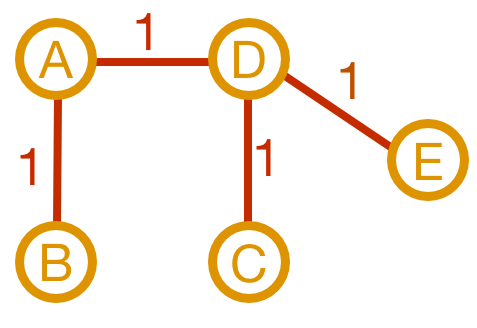
\includegraphics[width=0.4\textwidth]{tex/fig/graf7}
	\caption{Prim -- Krok 7.}
	\label{fig: g7}
\end{figure}
\newpage